\chapter{Deep Q-Learning}

With algorithms such as Q-Learning, one can learn by choosing the actions and observing their results directly in the environment. Put into an ACC context, it is possible to learn an acting policy in a simulated highway system by taking ac- tions on the cars? brakes and throttle, and observing the results. The policy obtained can be used as a longitudinal controller to safely follow a preceding vehicle.

\section{General Architecture}

Our system follows the basic RL structure. The agent performs an action $A_t$ given state $S_t$ under policy $\pi$. The agent receives the state as feedback from the environment and gets the reward $r_t$ for the action taken. The state feedback that the agent takes from sensors consists of the velocities of the neighboring vehicles $v_{veh}[]$ and the relative positions of the neighboring vehicles to the ego vehicle $dist_{veh}[]$. Possible action that agent can choose is among 4 levels of accelerations, 4 levels of decelerations and keeping the current speed. The goal of our proposed Adaptive Cruise System is to maximize the expected accumulated reward called "value function" that will be received in the future within an episode. Using the simulations, the agent learns from interaction with environment episode-by-episode. One episode starts when the vehicle and road state information are detected. The vehicle drives on a standard circular track . If the distance between the ego vehicle and the front vehicle or the behind vehicle is less than the safety distance $dist_{safe}$, it is considered as a collision event. The episode ends if at least one of the following events occurs

\begin{itemize}

\item \textbf{Collision} The ego vehicle detects the distance with the vehicle in front or behind within $dist_{safe}$.

\item \textbf{Time Out} The ego vehicle failed to finished N laps within a specific time.

\item \textbf{Finishing} The ego vehicle successfully finished N laps within a specific time.

\item \textbf{Bump} The ego vehicle is turned over for some reason.

\item \textbf{Off Lane} The ego vehicle is out of lanes.

\end{itemize}

The ego vehicle continuously detect the vehicles around itself as shown in Fig \ref{fig:highway}. The vehicle $i$ ($i$ = 0,1,...,5) do not represent any specific vehicle but a detected vehicle in that area. For example, Vehicle 0 and Vehicle 1 represent vehicles in the left lane of the ego vehicle and Vehicle 0 is behind and Vehicle 1 is in front of it. When there are multiple vehicles in the same area, only the closest is remained. When there is no vehicle there, a fake and safe vehicle would be used to maintain the state structure, which would be described in more detail later.

\begin{figure}[h]
\centering
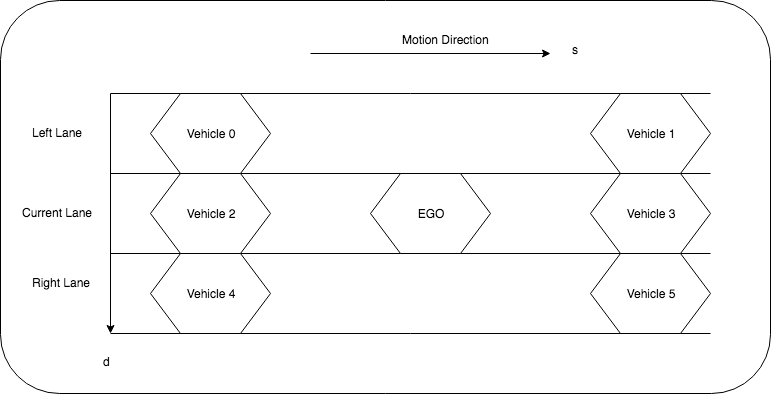
\includegraphics[width=0.5\textwidth]{figs/ch4/Highway-Display}
\caption{A general highway case display.}
\label{fig:highway}
\end{figure}

Once one episode ends, the next episode starts with the state of environment and the value function reset.


\section{Reinforcement Learning for Longitudinal Motion}

Reinforcement Learning (RL) is an interesting technique for the design of a longitudinal controller because it enables us to abstract from the complexity of car physics and dynamics that have an important computing cost. With algorithms such as Q-Learning, one can learn by choosing the actions and observing their results directly in the environment. Put into an ACC context, it is possible to learn an acting policy in a simulated highway system by taking actions on the cars? brakes and throttle, and observing the results. The policy obtained can be used as a longitudinal controller to safely follow a preceding vehicle.

To apply this RL framework, we first had to model the problem by defining the states, actions, goals and rewards. Our first approach was to use variables such as the position of a leading car and of a follower, their velocities and accelerations, etc. Clearly, this state definition put us up against the curse of dimensionality, and it became impossible to have a discrete state space precise enough to learn a valuable policy. We modified our state definition by consolidating numerous state variables. This allowed us to use a smaller discretization and to reach a better precision with only two variables. Since driving can be seen as a sequential decision problem, there is no problem in modeling it using a MDP and discrete state variables. As seen in section 7, part of our future works will be to implement techniques to better approximate the continuous aspects of the problem. For now, our discrete state space was built around a state definition containing variables similar to those used in [14] for a fuzzy logic controller, as we defined our states by the relative distance in time between two vehicles and by the difference between those distances at two consecutive steps.

As seen in Eq. (1) and Eq. (2), the time distance takes into ac- count the relative position between the two vehicles and also the velocity of the follower, while the differences of the time distance between two consecutive time steps gives a signal about the movement of the vehicles relative to each other (whether they are closing up since last step, or getting farther). The time distance is the main variable for identifying the follower?s position related to the secure distance, while the difference in time completes the Markovian signal, as it adds to the state definition an evaluation of the relative acceleration or deceleration. This relative movement between vehicles is needed to take an informed decision on the action to take at the next time step. Those actions were taken directly on the brakes or throttle (only one action per time step is chosen), closely simulating human interaction. The actions were discretized, according to a percentage of pressure on the pedal, from 0 to 100 by increments of 20.

The goal was defined as a secure distance to reach behind a pre- ceding vehicle. That distance was specified as a time range and was defined as 2 seconds (� 0.1 sec.), as it is a value often used as a se- cure distance in today?s ACC systems [2]. To reach the goal, we set the rewards accordingly, with a positive reward given when the ve- hicle was located in the specified time range. We also set negative rewards when wandering too far or too close from the time ratio we were looking for. The behavior the agent was supposed to learn was to reach the secure distance specified as the goal, and to stay in that range for as long as possible.

Those elements were put together in a RL framework, and the policy obtained, learned in a simulated environment, formed the core of our longitudinal controller. The environment, a simulated highway system built in previous work, featured complex car physics and dynamics as described in [9]. Since the simulation environment was using continuous time, we had to define the time interval at which action decisions would be taken. The action chosen at the specified time frame would be taken for the whole frame. To observe an accurate behavior of the vehicle, we had to set the time step between each action decision to a small value (50 milliseconds). But in such conditions, the observation of real vehicle acceleration needed many consecutive acceleration actions, a behavior that could not be learned in a decent time with normal state space exploration. To overcome this problem, we had to use a heuristic to speed up learning. The heuristic specified that every time the car was behind the desired time ratio, the best acceleration action known from experience was taken. By ignoring in that case the braking actions, this action selection technique directed rapidly the agent towards more rewarding locations of the state space.

\begin{figure}[h]
\centering
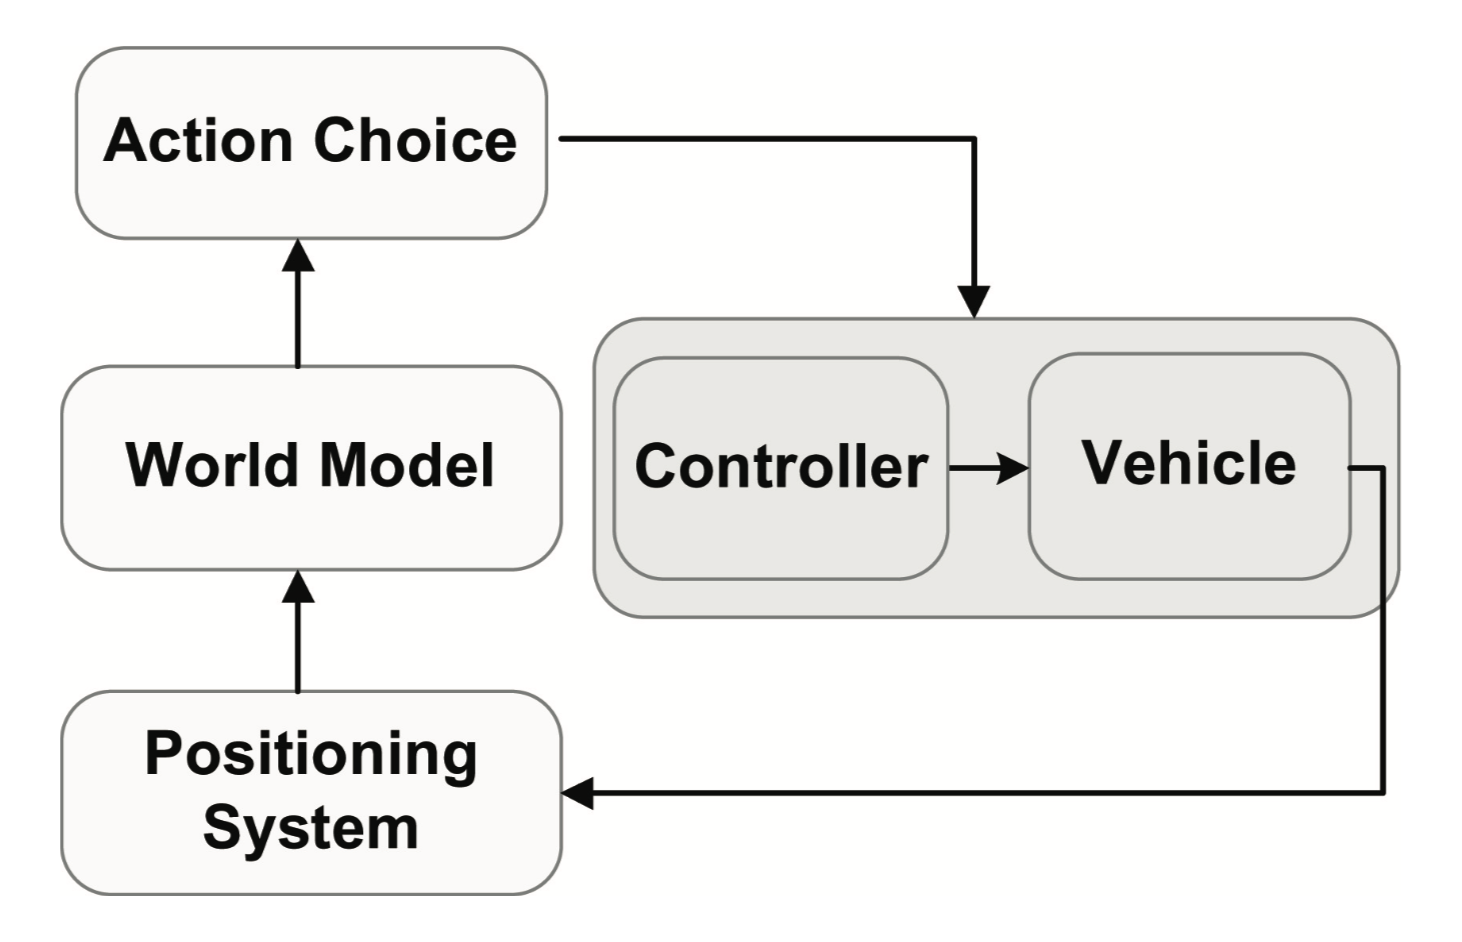
\includegraphics[width=0.5\textwidth]{figs/ch4/acc-drl}
\caption{Reinforcement applied on ACC system.}
\label{fig:acc-rl}
\end{figure}

Put into context, Figure 3 shows that using RL simplifies the de- sign of a longitudinal controller. The closed-loop controller takes as inputs the vehicle?s state as described earlier, and selects the appropriate action according to the policy that was learned. Such a technique is obviously simpler than the complex mathematical analysis needed to predict precise car physics and dynamics for act- ing, as our controller basically hides in a black box vehicle physics and dynamics. It is possible for the agent to learn the optimal behavior by taking driving actions and observing their results on the time distance and its difference between two time steps. In the next section, we will show results obtained by using this policy for longitudinal vehicle control. As drivers spend a great amount of their time in heavy traffic, such systems could reduce the risk of rear-end collisions and protect the drivers mentally by relieving them from stressful driving. (Source: [67])

\section{Reinforcement Learning for Lateral Motion}

Lateral motion control without longitudinal motion control hardly exists. Besides parking another good example of low speed combined longitudinal and lateral control is the traffic jam assist system. At speeds between zero and 40 or 60 km/h (depending on OEMs), the traffic jam assist system keeps pace with the traffic flow and helps to steer the car within certain constraints. It also accelerates and brakes autonomously. The system is based on the functionality of the adaptive cruise control with stop \& go, extended by adding the lateral control of steering and lane guidance. The function is based on the built-in radar sensors, a wide-angle video camera and the ultrasonic sensors of the parking system.


In this section, we describe the design of the Management layer and, more precisely, the design of the policy to select the most efficient and safest lane for each vehicle according to their current state and action.

Lane changes are stressful maneuvers for drivers, particularly during high-speed traffic flows.


\section{Q Learning}

Q-learning is one of the popular RL methods which searches for the optimal policy in an iterative fashion. Basically, the Q-value function $q_{\pi} (s, a)$ is defined as

\begin{equation}
q_\pi(s,a) = \mathbb{E}_\pi \left[ \sum _{k=0}^{\infty} \gamma ^k r_{t+k+1} | S_t = s, A_t = a \right]
\end{equation}

For the given state s and action a, where $r_t$ is the reward received at the time step t. The Q-value function is the expected sum of the future rewards which indicates how good the action $a$ is given the state $s$ under the policy of the agent $\pi$. The contribution to the Q-value function decays exponentially with the discounting factor $\pi$ for the rewards with far-off future. For the given Q-value function, the greedy policy is obtained as

\begin{equation} \label{eq:402}
\pi(s) = arg \max_a q_{\pi} (s, a) 
\end{equation}

One can show that for the policy in Eq. \ref{eq:402}, the following Bellman equation should hold,

\begin{equation}
q_\pi(s,a) = \mathbb{E}_\pi [r_{t+1} + \gamma \max_a q_\pi(S_{t+1},a) | S_t = s, A_t = a]
\end{equation}

In practice, since it is hard to obtain the exact value of $q_{\pi}(s, a)$ satisfying the Bellman equation, the Q-learning method uses the following update rule for the given one step backups $S_t$, $A_t$, $r_{t+1}$, $S_{t+1}$;

\begin{equation}
q_\pi(S_t,A_t) \gets q_\pi(S_t,A_t) + \alpha \left[r_{t+1} + \gamma \max_a q_\pi(S_{t+1},a) - q_\pi(S_t,A_t)\right]
\end{equation}

However, when the state space is continuous, it is impossible to find the optimal value of the state-action pair $q_{\pi} (s, a)$ for all possible states. To deal with this problem, the DQN method was proposed, which approximates the state-action value function q(s, a) using the DNN, i.e., $q(s, a) = q_\theta(s, a)$ where $\theta$ is the parameter of the DNN. The parameter $\theta$ of the DNN is then optimized to minimize the squared value of the temporal difference error $\delta_t$

\begin{equation} \label{eq:delta-1}
\delta_t = r_{t+1} + \gamma \max_{a^ \prime} q_\theta(S_{t+1},a^ \prime) - q_\theta(S_t,A_t)
\end{equation}

For better convergence of the DQN, instead of estimating both $q(S_t,A_t)$ and $q(S_{t+1},a^ \prime)$ in  Eq. (4.5), we approximate $q(St,At)$ and $q(S_{t+1},a^ \prime)$ using the Q-network and the target network parameterized by $\theta$ and $\theta^{\prime}$, respectively. The update of the target network parameter $\theta^{\prime}$, is done by cloning Q-network parameter $\theta$, periodically. Thus, Eq. \ref{eq:delta-1} becomes

\begin{equation}
\delta_t = r_{t+1} + \gamma \max_{a^ \prime} q_{\theta^{\prime}}(S_{t+1},a^ \prime) - q_\theta(S_t,A_t)
\end{equation}

To speed up convergence further, replay memory is adopted to store a bunch of one step backups and use a part of them chosen randomly from the memory by batch size. The backups in the batch is used to calculate the loss function L which is given by

\begin{equation}
L = \sum_{t\in B_{replay}}\delta_t^2
\end{equation}

where $B_{replay}$ is the backups in the batch selected from replay memory. Note that the optimization of parameter $\theta$ for minimizing the loss $L$ is done through the stochastic gradient decent method.



One of the most basic and popular methods to estimate action-value functions is the \emph{Q-learning} algorithm. It is model-free online off-policy algorithm, whose main strength is that it is able to compare the expected utility of the available actions without requiring a model of the environment. Q-learning works by learning an action-value function that gives the expected utility of taking a given action in a given state and following a fixed policy thereafter.

A value function estimates what is good for an agent over the long run. It estimates the expected outcome from any given state, by summarizing the total amount of reward that an agent can expect to accumulate into a single number. Value functions are defined for particular policies.

The \emph{state value function} (or V-function), is the expected return when starting in state $s$ and following policy $\pi$ thereafter~\citep{Sutton1998RL},
%
\begin{equation}
V^\pi(s) = \mathbb{E}_\pi \left[R_t | s_t = s \right]
\end{equation}

The \emph{action value function} (or Q-function), is the expected return after selecting action $a$ in state $s$ and then following policy $\pi$,
%
\begin{equation}
q^\pi(s,a) = \mathbb{E}_\pi \left[ R_t | s_t = s, a_t = a \right]
\end{equation}

The \emph{optimal value function} is the unique value function that maximizes the value of every state, or state-action pair,
%
\begin{eqnarray}
Q^*(s,a) & = & \max\limits_\pi Q^\pi(s,a), \forall s \in \mathcal{S}, a \in \mathcal{A}
\end{eqnarray}

An \emph{optimal policy} $\pi^*(s,a)$ is a policy that maximizes the action value function from every state in the MDP,
%
\begin{equation}
    \pi^*(s,a) = \argmax_\pi Q^\pi(s, a)
\end{equation}

The update rule uses action-values and a built-in max-operator over the action-values of the next state in order to update $Q(s_t, a_t)$ as follows,

\begin{equation}
Q(s_t,a_t) \gets Q(s_t,a_t) + \alpha \left[r_{t+1} + \gamma \max_a Q(s_{t+1},a) - Q(s_t,a_t)\right]
\end{equation}

The agent makes a step in the environment from state $s_t$ to $s_{t+1}$ using action $a_t$ while receiving reward $r_t$. The update takes place on the action-value $a_t$ in the state $s_t$ from which this action was executed. This version of Q-learning works well for tasks with a small a state-space, since it uses arrays or tables with one entry for each state-action pair.

In this project the policy is using the \textbf{$\epsilon$-greedy} policy:

\begin{itemize}

    \item \textbf{$\epsilon$-greedy.} Selects the best action for a proportion
        $1 - \epsilon$ of the trials, and another action is randomly selected (with
        uniform probability) for a proportion,
        
        \begin{equation}
            \pi_{\epsilon}(s) = \left\{
             \begin{array}{lr}
                 \pi_{\textrm{rand}}(s,a) & \text{if } rand() < \epsilon\\
                 \pi_{\textrm{greedy}}(s,a) & \text{otherwise}
             \end{array}
           \right.
        \end{equation}

        where $\epsilon \in [0, 1]$ and $rand()$ returns a random number from a uniform distribution $\in [0, 1]$.

\end{itemize}

\section{Policy Representation}

A policy is a mapping between a state space S and an action space $A$, i.e., $\pi(s) : S \to A$. For our framework, $S$ is a continuous space that describes the state of the ego vehicle and neighboring vehicles. The action space $A$ is represented by a 27 sized 1D discrete space where each action specifies a behavior the ego vehicle could do. The following sections provide further details about the policy representation.

\subsection{State}

A state $s$ consists of features describing the state of the ego vehicle and relative positions and velocities with its neighboring vehicles. The state is represented by its pose q and velocity q?, where q records the positions of the center of mass of each link with respect to the root and q? records the center of mass velocity of each link. The terrain features, $T$ , consist of a 1D array of samples from the terrain height- field, beginning at the position of the root and spanning 10 m ahead. All heights are expressed relative to the height of the terrain immediately below the root of the character. The samples are spaced 5 cm apart, for a total of 200 height samples. Combined, the final state representation is 283-dimensional. Figure 5 and 6 illustrate the character and terrain features.

\subsection{Actions}

A total of 27 controller parameters serve to define the available policy actions. These include specifications of the target spine curvature as well as the target joint angles for the shoulder, elbow, hip,

\subsection{Reward Function}

Unlike video games, the reward should be appropriately defined by a system designer in Adaptive Cruise System. As mentioned, the reward function determines the behavior of the adaptive cruise. Hence, in order to ensure the reliability of the adaptive cruise control, it is crucial to use the properly defined reward function. In our model, there is conflict between two intuitive objectives for cruise control; 1) collision should be avoided no matter what happens and 2) the vehicle should get out of the risky situation quickly. If it is unbalanced, the agent becomes either too conservative or reckless. Therefore, we should use the reward function which balances two conflicting objectives. Taking this into consideration, we propose the following reward function

\begin{equation} \label{eq:reward-func}
r_t = \alpha * vel_{ego} + \beta * (s_{ego} - s_{behind}) + r
\end{equation}

where $v_t$ is the velocity of the vehicle at the time step $t$, decel is difference between $v_t$ and $v_{t1}$ and 1(x = y) has a value of 1 if the statement inside is true and 0 otherwise. The first term ?(?(pedposx ? vehposx)2 + ?)decel in the reward function prevents the agent from braking too early by giving penalty proportional to squared distance between the vehicle and pedestrian. It guides the vehicle to drive without deceleration if the pedestrian is far from the vehicle. On the other hand, the term ?(?vt2 + ?)1(St = bump) indicates the penalty that the agent receives when the accident occurs. Note that this penalty is a function of the vehicle?s velocity, which reflects the severe damage to the pedestrian in case of high velocity at collision. Without such dependency on the velocity, the agent would not reduce the speed in situation when the accident is not avoidable. The constants $\alpha$, $\beta$, $\phi$ and $\psi$ are the weight parameters that controls the trade-off between two objectives.

\subsection{Relay Memory}

In reinforcement learning (RL), the agent observes a stream of experiences and uses each experience to update its internal beliefs. For example, an experience could be a tuple of (state, action, reward, new state), and the agent could use each experience to update its value function via TD-learning. In standard RL algorithms, an experience is immediately discarded after it?s used for an update. Recent breakthroughs in RL leveraged an important technique called experience replay (ER), in which experiences are stored in a memory buffer of certain size; when the buffer is full, oldest memories are discarded. At each step, a random batch of experiences are sampled from the buffer to update agent?s parameters. The intuition is that experience replay breaks the temporal correlations and increases both data usage and computation efficiency Lin (1992).

Combined with deep learning, experience replay has enabled impressive performances in AlphaGo Silver et al. (2016), Atari games Mnih et al. (2015), etc. Despite the apparent importance of having a memory buffer and its popularity in deep RL, relatively little is understood about how basic characteristics of the buffer, such as its size, affect the learning dynamics and performance of the agent. In practice, a memory buffer size is determined by heuristics and then is fixed for the agent.

As mentioned in the previous section, the adaptive cruise system should learn both of the conflicting objectives. However, when we train the DQN with the reward function in Eq. \ref{eq:reward-func}, we find that the learning performance is not stable since collision events rarely happen and thus there remains only a few one-step backups associated with the collisions in the replay memory. As a result, the probability of picking such one-step backups is small and the DQN does not have enough chance to learn to avoid accidents in practical learning stage. To solve this issue, we propose so called "trauma" memory which is used to store only the one-step backups for the rare events (e.g., collision events in our scenario). While the one step backups are randomly picked from the replay memory, some fixed number of backups associated with the collision events are randomly selected from the trauma memory and used for training together. In other words, with the trauma memory, the loss function $L$ is modified to

equation ... (Autonomous Braking System via Deep Reinforcement Learning)

where $B_{trauma}$ is the backups randomly picked from trauma memory. Trauma memory persistently reminds the agent of the memory on the accidents regardless of the current policy, thus allowing the agent to learn to maintain speed and avoid collisions reliably.


\section{Deep Neural Network Layer}

Many of the successes in DRL have been based on scaling up prior work in RL to high-dimensional problems. This is due to the learning of low-dimensional feature representations and the powerful function approximation properties of neural networks. By means of representation learning, DRL can deal efficiently with the curse of dimensionality, unlike tabular and traditional non-parametric methods [15]. For instance, convolutional neural networks (CNNs) can be used as components of RL agents, allowing them to learn directly from raw, high-dimensional visual inputs. In general, DRL is based on training deep neural networks to approximate the optimal policy ??, and/or the optimal value functions $V^\star$, $Q^\star$ and $A^\star$.

Although there have been DRL successes with gradient free methods [37, 23, 64], the vast majority of current works rely on gradients and hence the backpropagation algorithm [162, 111]. The primary motivation is that when available, gradients provide a strong learning signal. In reality, these gradients are estimated based on approximations, through sampling or otherwise, and as such we have to craft algorithms with useful inductive biases in order for them to be tractable.The other benefit of backpropagation is to view the optimization of the expected return as the optimization of a stochastic function [121, 46]. This function can comprise of several parts?models, policies and value functions?which can be combined in various ways. The individual parts, such as value functions, may not directly optimize the expected return, but can instead embody useful information about the RL domain. For example, using a differentiable model and policy, it is possible to forward propagate and backpropagate through entire rollouts; on the other hand, inacuracies can accumulate

Convolutional Neural Networks, or CNNs, are a special type of neural network that has a known grid-like topology. Like most other neural networks they are trained with a variant of the back-propagation algorithm. CNN's strength is pattern recognition directly from pixels of images with minimal processing. We use a convolutional network as a function mapping the preprocessed images to Q values, since the actions are highly based on what would be seen as pixel matrix.

\begin{figure}[h]
\centering
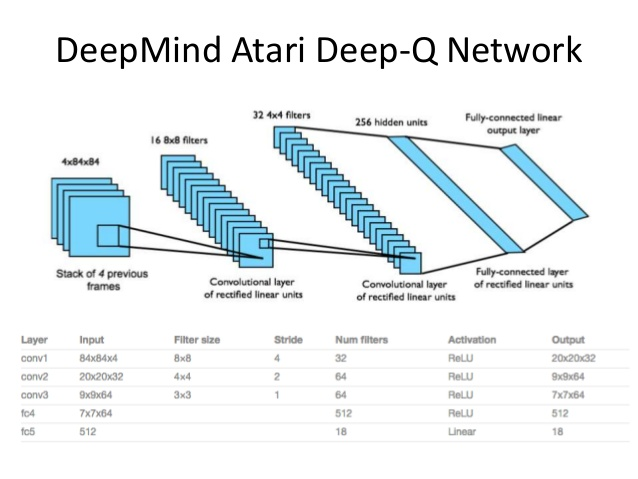
\includegraphics[width=0.5\textwidth]{figs/ch4/deepmind-atari-network}
\caption{Deep Neural Network model from DeepMind paper.}
\end{figure}



\vfill
